%\documentclass[aps,prl,preprint,groupedaddress]{revtex4-1}
%\documentclass[aps,prl,preprint,superscriptaddress]{revtex4-1}
\documentclass[aps,prl, reprint,superscriptaddress]{revtex4-1}
\newcommand{\SSC}{S/S_{c}}
\usepackage{graphicx}
% You should use BibTeX and apsrev.bst for references
% Choosing a journal automatically selects the correct APS
% BibTeX style file (bst file), so only uncomment the line
% below if necessary.
%\bibliographystyle{apsrev4-1}

\begin{document}

% Use the \preprint command to place your local institutional report
% number in the upper righthand corner of the title page in preprint mode.
% Multiple \preprint commands are allowed.
% Use the 'preprintnumbers' class option to override journal defaults
% to display numbers if necessary
%\preprint{}

%Title of paper
\title{The Magnetorotational Instability Prefers Three Dimensions}

% repeat the \author .. \affiliation  etc. as needed
% \email, \thanks, \homepage, \altaffiliation all apply to the current
% author. Explanatory text should go in the []'s, actual e-mail
% address or url should go in the {}'s for \email and \homepage.
% Please use the appropriate macro foreach each type of information

% \affiliation command applies to all authors since the last
% \affiliation command. The \affiliation command should follow the
% other information
% \affiliation can be followed by \email, \homepage, \thanks as well.
\author{Jeffrey~S.~Oishi}
\email[]{joishi@bates.edu}
\affiliation{Bates College Department of Physics and Astronomy, Lewiston, ME 04240}

\author{Geoffrey~M.~Vasil}
\affiliation{University of Sydney School of Mathematics and Statistics, Sydney, NSW, Australia}
\author{Morgan Baxter}
\affiliation{Bates College Department of Physics and Astronomy, Lewiston, ME 04240}
\author{Andrew Swan}
\affiliation{Faculty of Mathematics, Cambridge University, Cambridge, United Kingdom}
\author{Keaton~J.~Burns}
\affiliation{Center for Computational Astrophysics, Flatiron Institute, New York, NY 10010}
\affiliation{Massachusetts Institute of Technology Department of Physics, Cambridge, MA 02139}
\author{Daniel~Lecoanet}
\affiliation{Princeton Center for Theoretical Science and Princeton University Department of Astrophysical Sciences, Princeton, NJ 08544}
\author{Benjamin~P.~Brown}
\affiliation{University of Colorado Laboratory for Atmospheric and Space Physics and Department of Astrophysical and Planetary Sciences, Boulder, CO 80309}

% 
%\homepage[]{Your web page}
%\thanks{}
%\altaffiliation{}


%Collaboration name if desired (requires use of superscriptaddress
%option in \documentclass). \noaffiliation is required (may also be
%used with the \author command).
%\collaboration can be followed by \email, \homepage, \thanks as well.
%\collaboration{}
%\noaffiliation

\date{\today}

\begin{abstract}
Write abstract last.
\end{abstract}

% insert suggested PACS numbers in braces on next line
\pacs{}
% insert suggested keywords - APS authors don't need to do this
%\keywords{}

%\maketitle must follow title, authors, abstract, \pacs, and \keywords
\maketitle

% body of paper here - Use proper section commands
% References should be done using the \cite, \ref, and \label commands

\section{Introduction}
\label{sec:intro}

\begin{itemize}
\item 3D $\to$ dynamo
\item stars, NSSL
\item experiments
\end{itemize}

\section{Method}
\label{sec:method}

We solve the linearized magnetohydrodynamic equations in a frame rotating with angular frequency $\Omega$. The Navier-Stokes equations is in a fairly standard form,
\begin{equation}
  \label{eq:ns}
  \frac{D \mathbf{v}}{Dt} - f \hat{z} \times \mathbf{v} + S v_x \hat{z} + \mathbf{\nabla}{p} + \nu \mathbf{\nabla} \times \mathbf{\omega} = 0,
\end{equation}
where $\omega = \mathbf{\nabla} \times \mathbf{v}$ is the vorticity, $f = 2 \Omega$ is the Coriolis parameter, and $S$ is the background shear rate. $Df/Dt = \partial f/\partial t + S x \partial f/\partial y$ is the advective derivative including the background linear shear velocity.  We write the induction equation in terms of the $x$ component of the magnetic field,
\begin{equation}
  \label{eq:Bx}
  \frac{D B_x}{Dt} - B_0 \partial_z v_x + \eta (\partial_y J_z - \partial_z J_y) = 0
\end{equation}
and the $x$ component of the current density,
\begin{equation}
  \label{eq:Jx}
  \frac{D J_x}{Dt} - B_0 \partial_z \omega_x + S \partial_z B_x - \eta \nabla^2 J_x = 0
\end{equation}
We explicitly enforce the divergence constraint on the incompressible velocity field $v$ and the magnetic field,
\begin{equation}
  \label{eq:divu}
  \mathbf{\nabla} \cdot \mathbf{v} = \mathbf{\nabla} \cdot \mathbf{B} = 0.
\end{equation}
The magnetic field is expressed in Alfven units, $\mathbf{B} = \mathbf{B_*}/\sqrt{\mu_0 \rho}$.
We consider the behavior of the MRI in a vertically ($z$) and horizontally ($y$) periodic channel of width $L_x = \pi$. The walls at $x = \pm L_x/2$ are perfectly conducting and stress-free. The MRI is a weak-field instability; in the invisicd, ideal case the critical shear rate for instability in two dimensions is given by
\begin{equation}
  \label{eq:Sc}
  S_c = \frac{-\pi^2 B^2}{f d^2}.
\end{equation}
Here, we use $\SSC$ as our control parameter. 

We solve equations~(\ref{eq:ns})--~(\ref{eq:divu}) by assuming harmonic perturbations in $y$ and $z$, $f = \hat{f}(x) e^{i(k_y y + k_z z) + \gamma t}$. This reduces to an eigenvalue problem in $x$, which we solve using the \emph{Dedalus} pseudospectral framework. The advantage of this particular form is that it can be expressed as a set of ten first-order equations with Dirichlet boundary conditions for either no-slip or stress-free boundary conditions. 

Our interest is in nearly ideal ($\eta = 0$), inviscid ($\nu = 0$) conditions; we thus set $\eta=\nu=10^{-5}$, though we have confirmed our main results are insensitive to this particular value. 

\section{Results}
\label{sec:results}
Our most surprising result is that at very small values of supercriticality, the fastest growing mode is not axisymmetric. Figure~\ref{fig:growth_rate} shows the growth rates for three values of $\SSC$. At $\SSC = 1.01$, the maximum growth rate is $(k_y, k_z) \simeq (0.263, 0.447)$. 

\begin{figure}[h]
  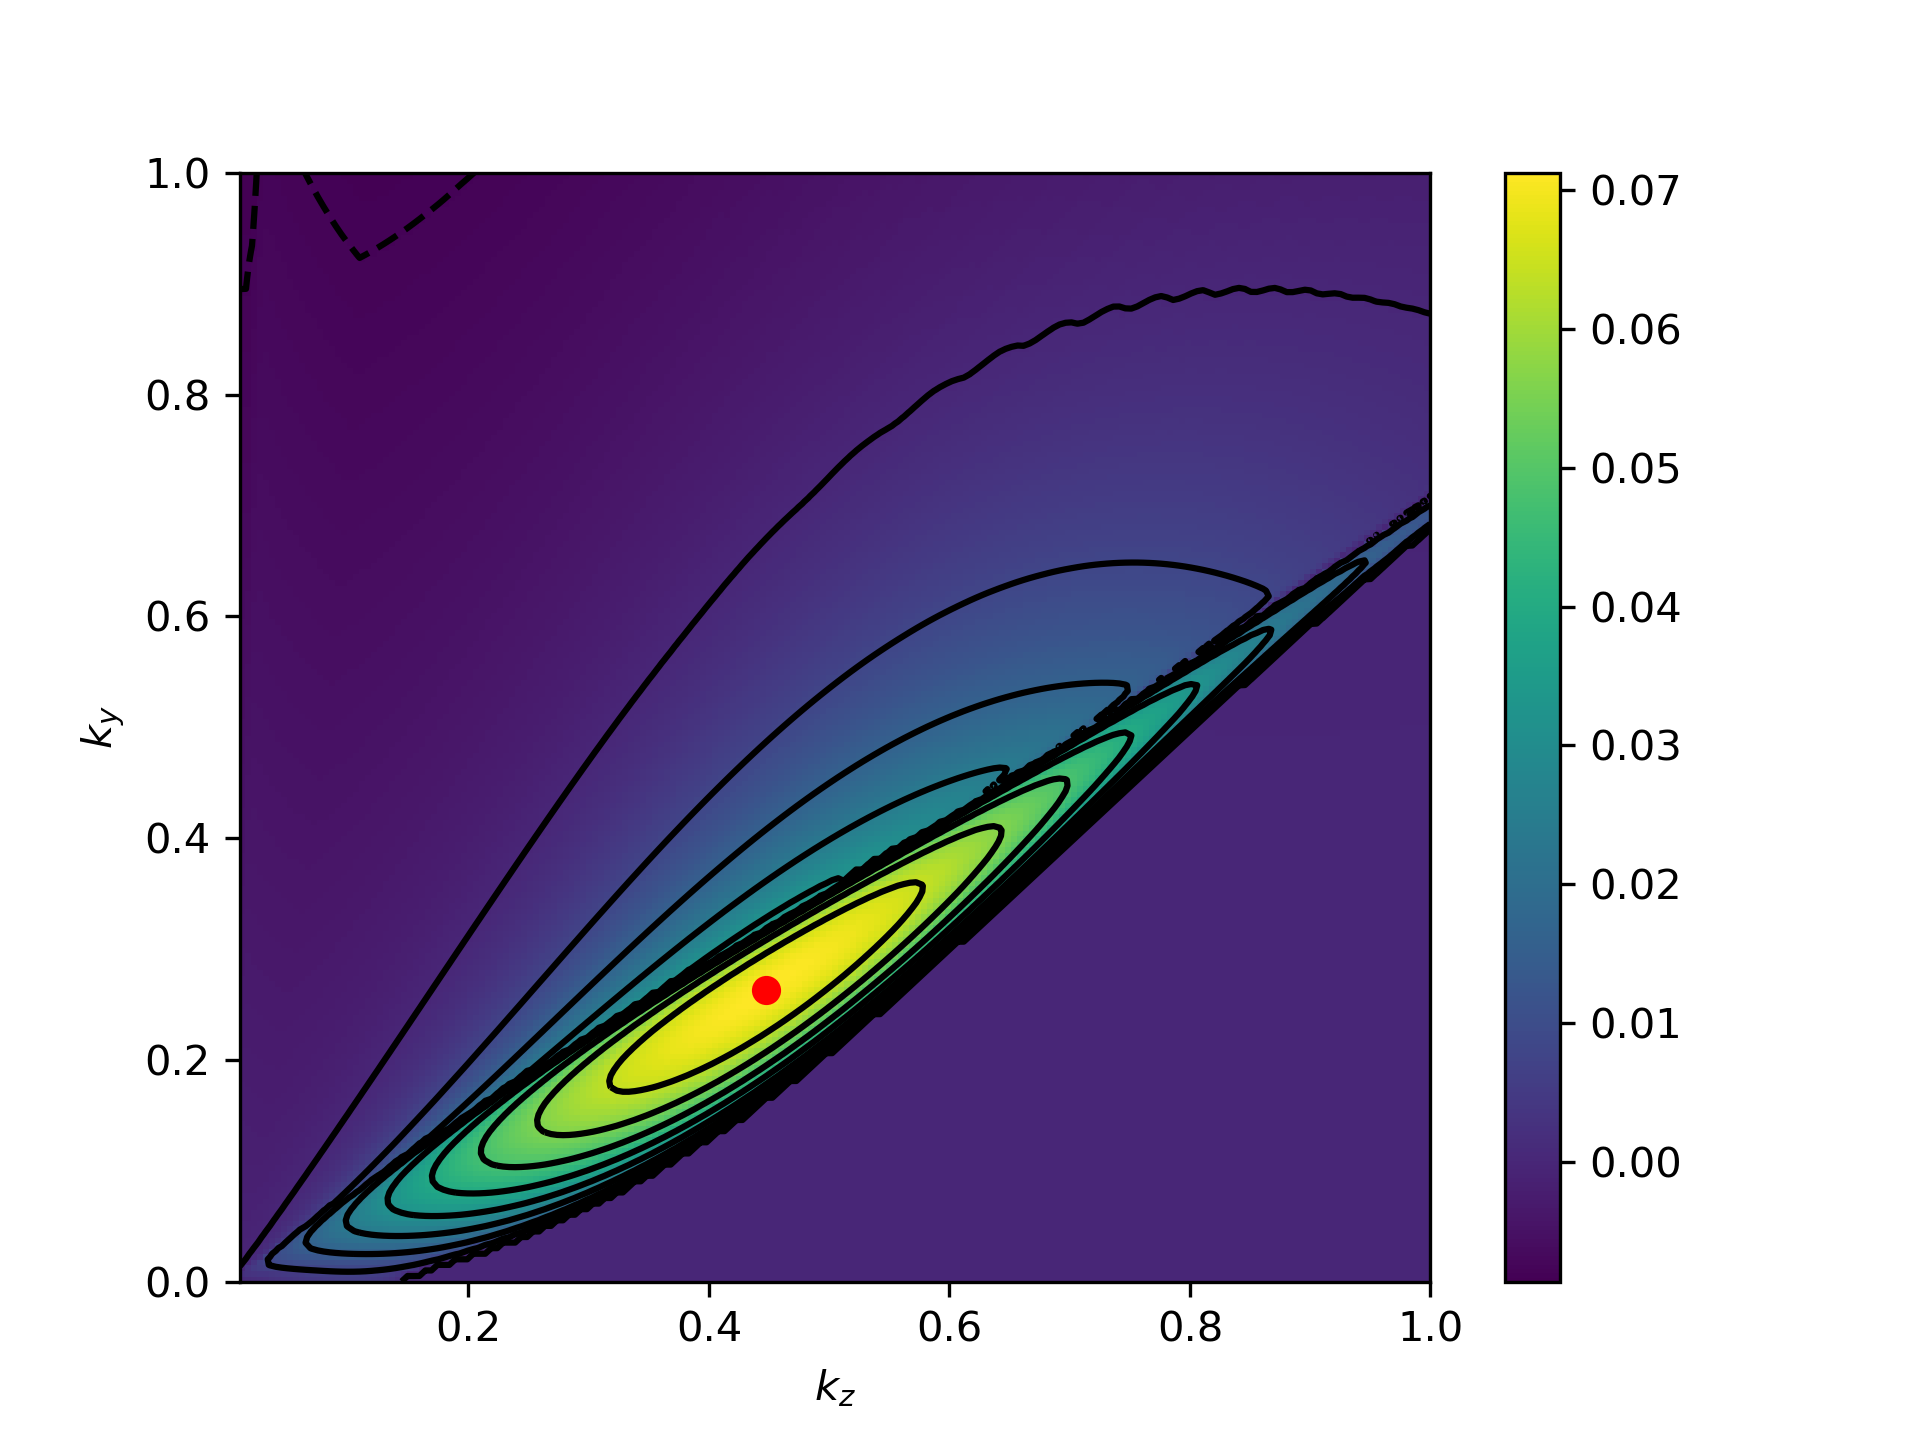
\includegraphics[width=\columnwidth]{run_11_output_growthrates.png}
  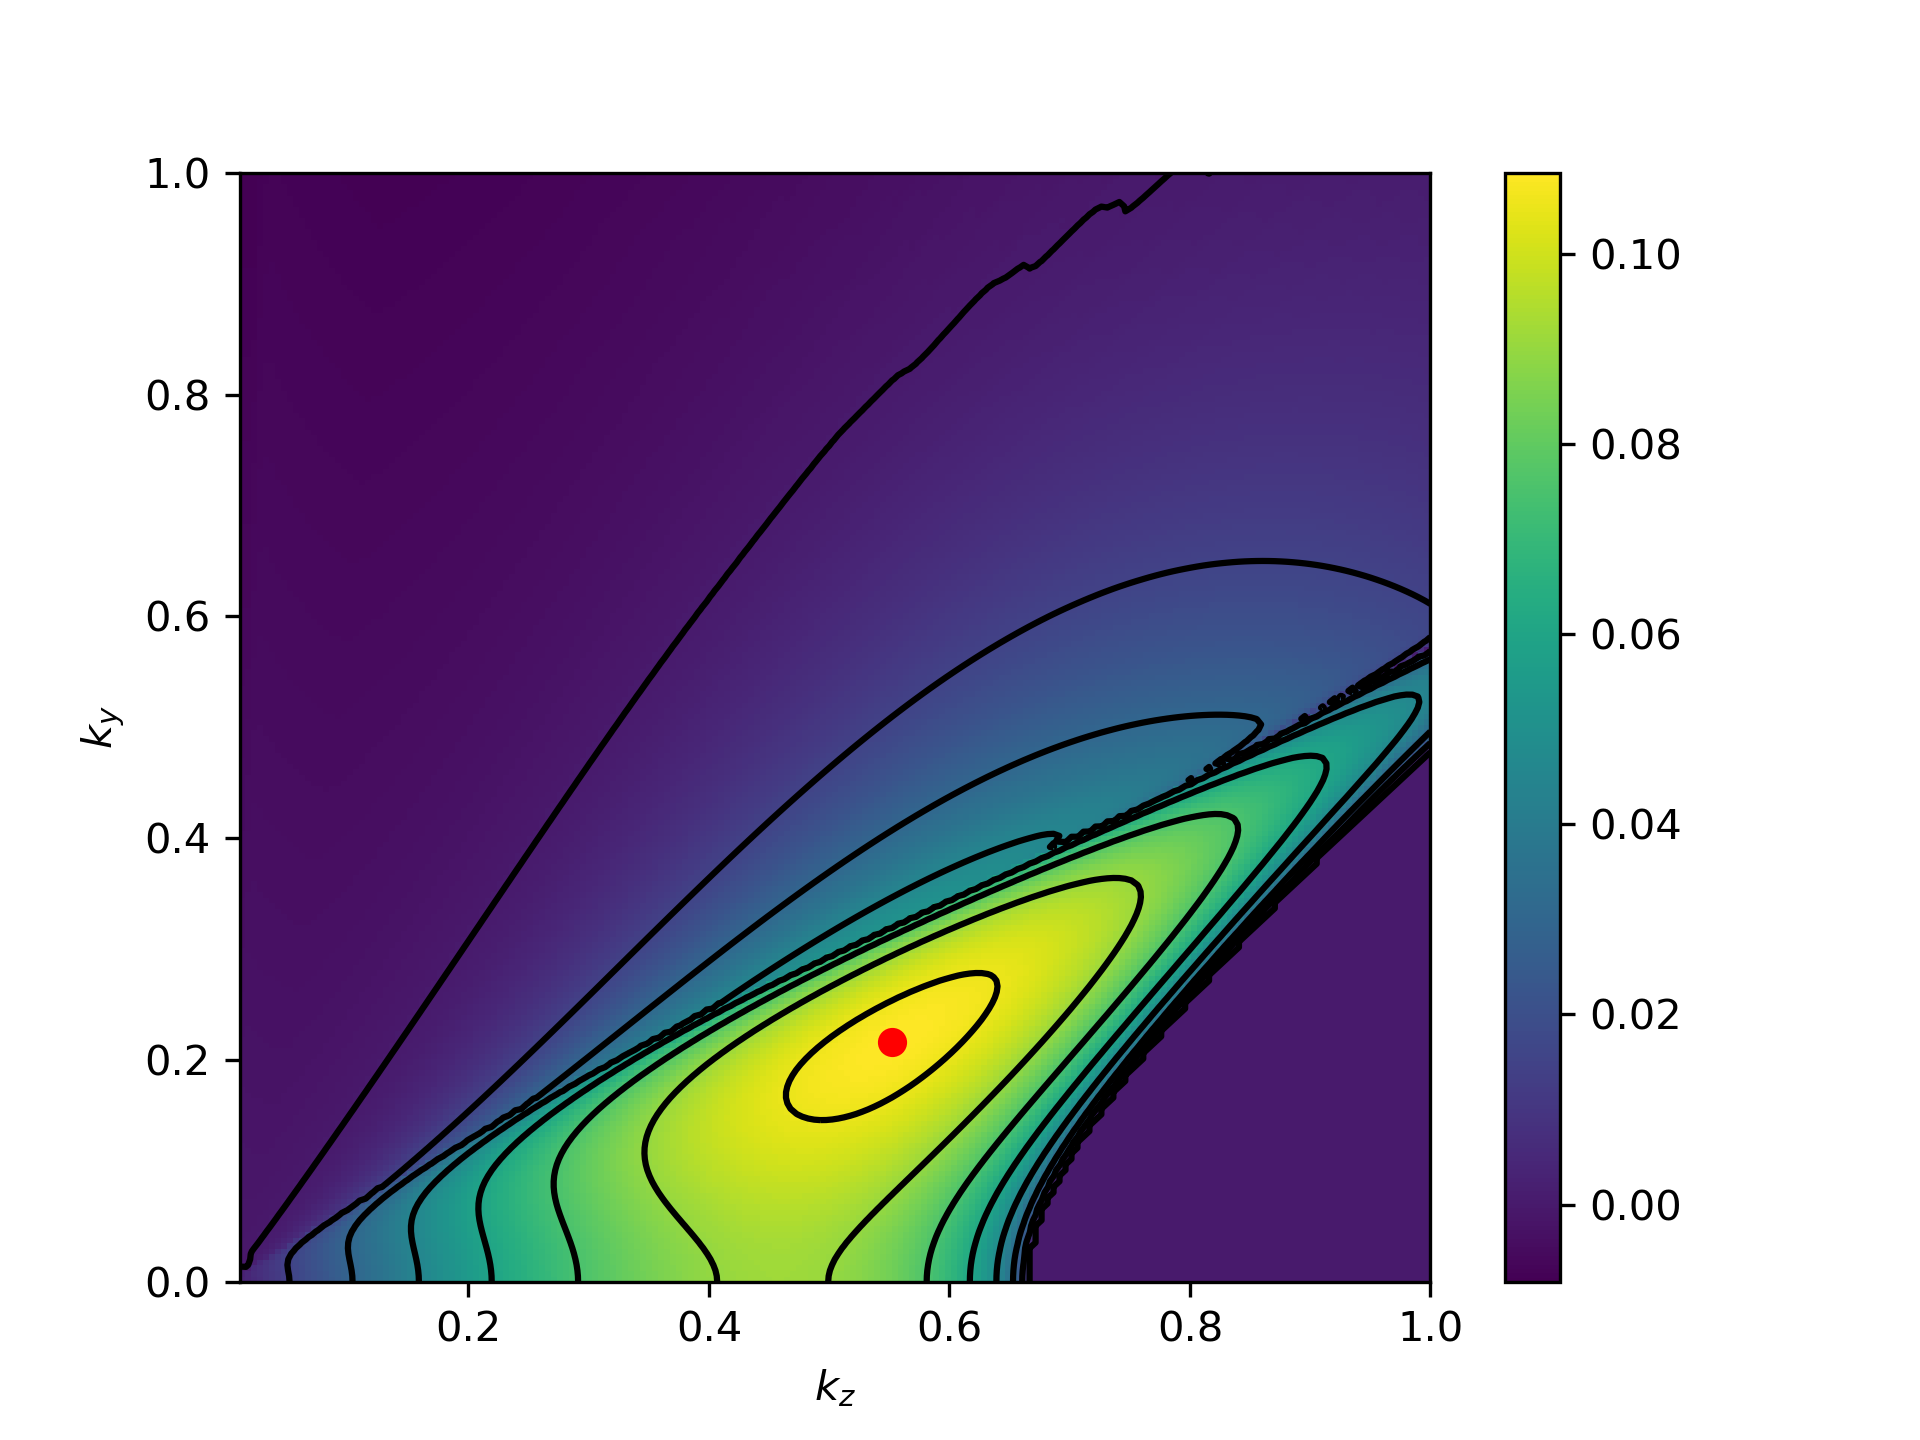
\includegraphics[width=\columnwidth]{run_12_output_growthrates.png}
  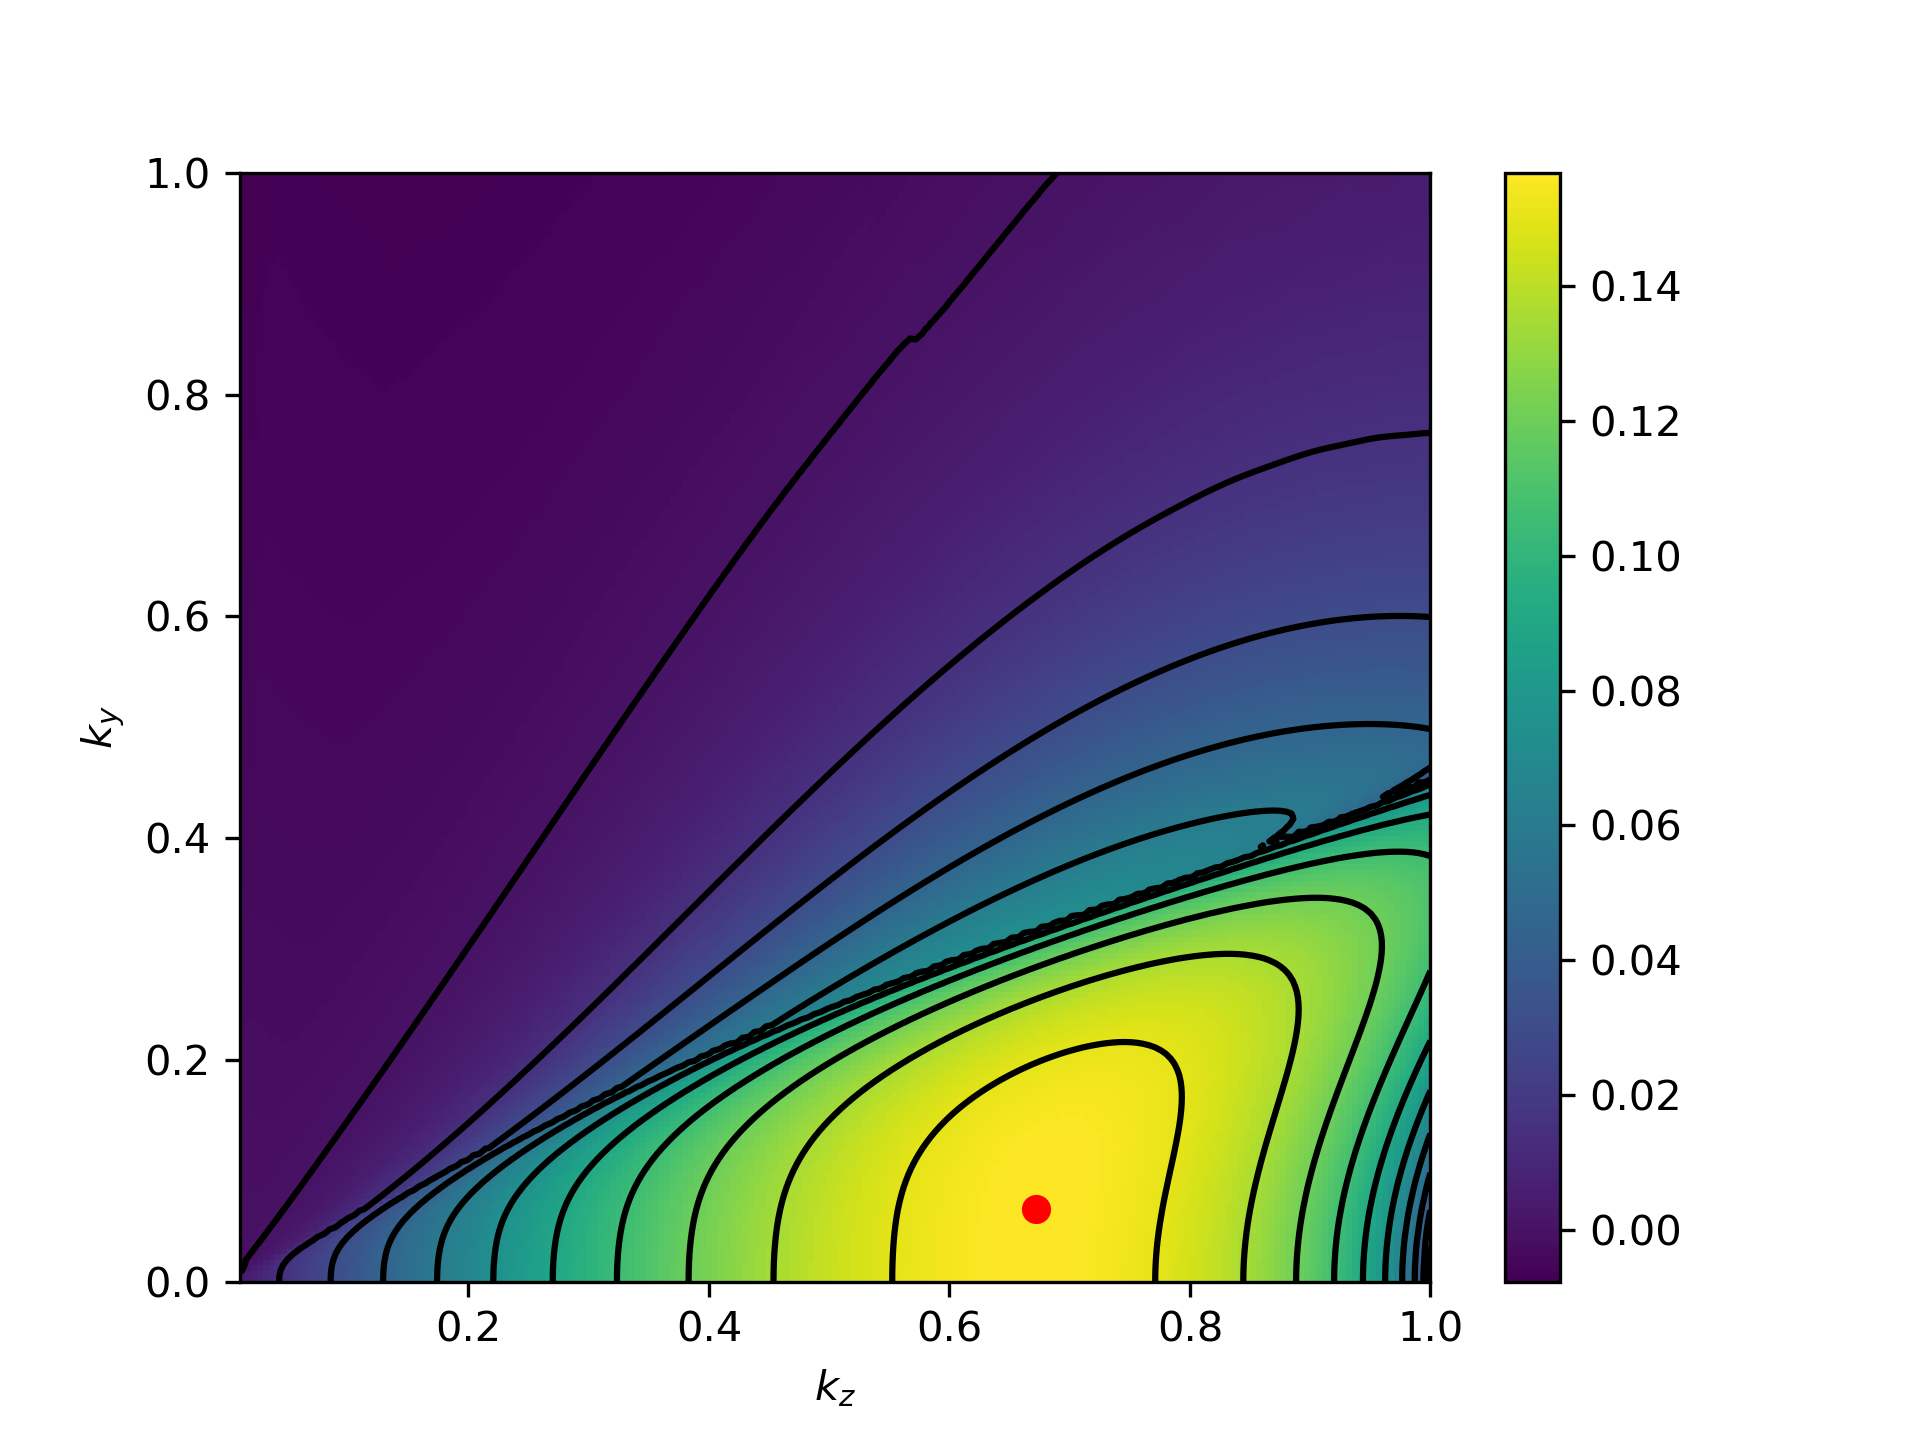
\includegraphics[width=\columnwidth]{run_13_output_growthrates.png}
  \caption{Growth rate as a function of $k_z$ and $k_y$. The maximum growth rate is far from $k_y = 0$, indicating the MRI is most unstable in a fully three-dimensional configuration.}
  \label{fig:growth_rate}
\end{figure}

Numerical simulations have consistently axisymmetric modes dominating early evolution of the MRI (cite Stone 95, etc) before parasitic modes cause a breakdown into MHD turbulence. However, our results recover this limit, as $\SSC$ becomes large. Figure~\ref{fig:alpha} plots $\alpha = \arctan k_y/k_z$ as  function of $\SSC$. Above $\SSC \gtrsim 2$, $\alpha$ is zero, indicating that axisymmetric modes have the fastest growth rates.

\begin{figure}[h]
  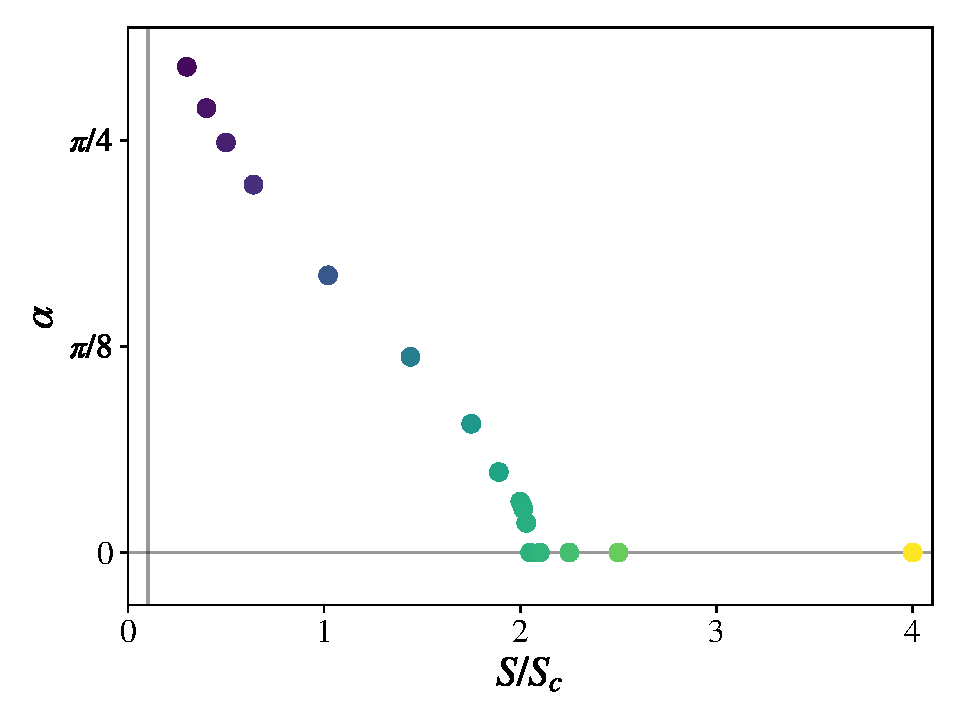
\includegraphics[width=\columnwidth]{alpha_vs_ssc_grid.pdf}
  \caption{Angle $\alpha$ vs $\SSC$. Stability limit is at $\SSC \simeq 0.102$}
  \label{fig:alpha}
\end{figure}
\section{Non-Normality}
\label{sec:non-normality}

\section{Speculations}
\label{sec:speculations}

\begin{itemize}
\item non-normal and $k_y$ even when $\alpha = 0$ implies important role for linear dynamics at early times. 
\item Following Squire + Bhattacharjee, this suggests that important stellar layers may in fact be driven by linear dynamics
\item why is MRI non-oscillatory when hydro shear is oscil or stable?
\end{itemize}
The linear operator for the MRI, like other shearing systems, is non-normal. 
%If in two-column mode, this environment will change to single-column
% format so that long equations can be displayed. Use
% sparingly.
%\begin{widetext}
% put long equation here
%\end{widetext}

% figures should be put into the text as floats.
% Use the graphics or graphicx packages (distributed with LaTeX2e)
% and the \includegraphics macro defined in those packages.
% See the LaTeX Graphics Companion by Michel Goosens, Sebastian Rahtz,
% and Frank Mittelbach for instance.
%
% Here is an example of the general form of a figure:
% Fill in the caption in the braces of the \caption{} command. Put the label
% that you will use with \ref{} command in the braces of the \label{} command.
% Use the figure* environment if the figure should span across the
% entire page. There is no need to do explicit centering.

% \begin{figure}
% \includegraphics{}%
% \caption{\label{}}
% \end{figure}

% Surround figure environment with turnpage environment for landscape
% figure
% \begin{turnpage}
% \begin{figure}
% \includegraphics{}%
% \caption{\label{}}
% \end{figure}
% \end{turnpage}

% tables should appear as floats within the text
%
% Here is an example of the general form of a table:
% Fill in the caption in the braces of the \caption{} command. Put the label
% that you will use with \ref{} command in the braces of the \label{} command.
% Insert the column specifiers (l, r, c, d, etc.) in the empty braces of the
% \begin{tabular}{} command.
% The ruledtabular enviroment adds doubled rules to table and sets a
% reasonable default table settings.
% Use the table* environment to get a full-width table in two-column
% Add \usepackage{longtable} and the longtable (or longtable*}
% environment for nicely formatted long tables. Or use the the [H]
% placement option to break a long table (with less control than 
% in longtable).
% \begin{table}%[H] add [H] placement to break table across pages
% \caption{\label{}}
% \begin{ruledtabular}
% \begin{tabular}{}
% Lines of table here ending with \\
% \end{tabular}
% \end{ruledtabular}
% \end{table}

% Surround table environment with turnpage environment for landscape
% table
% \begin{turnpage}
% \begin{table}
% \caption{\label{}}
% \begin{ruledtabular}
% \begin{tabular}{}
% \end{tabular}
% \end{ruledtabular}
% \end{table}
% \end{turnpage}

% Specify following sections are appendices. Use \appendix* if there
% only one appendix.
%\appendix
%\section{}

% If you have acknowledgments, this puts in the proper section head.
%\begin{acknowledgments}
% put your acknowledgments here.
%\end{acknowledgments}

% Create the reference section using BibTeX:
\bibliography{basename of .bib file}

\end{document}
%
% ****** End of file apstemplate.tex ******

